\documentclass{labreport}

\begin{document}

\labtitle
    {4}
    {Empirical Study of Dynamic Programming and Shortest Path Algorithms: Dijkstra vs Floyd-Warshall}
    {Student}
    {Covali Ilie, st. gr. FAF-243}
    {asist. univ. Fistic Cristofor}

\tableofcontents
\newpage

\lstset{style=python}

\section{Introduction and Motivation}

Shortest-path computation in weighted graphs is a foundational topic in computer science, with practical uses in network routing, transport systems, and game navigation. In practice, the best algorithm depends on the exact task: whether we need distances from one source or between all pairs, how dense the graph is, and what memory budget is available.

This laboratory compares two classic methods: Dijkstra and Floyd-Warshall. Dijkstra is commonly used for single-source shortest paths, while Floyd-Warshall solves the all-pairs version through dynamic programming. Even though their asymptotic behavior is well known, measured performance still depends on representation choices and implementation overhead. By evaluating both methods on graphs of increasing size and different densities, we can connect theory with observed behavior.

The goal is to build an experimental framework that captures practical performance, not just produce two implementations. Besides runtime, we track operation counters and memory use, then analyze how each metric scales with input size.

\section{Algorithm Design and Implementation}

\subsection{The Algorithms}

Dijkstra's algorithm maintains tentative distances in a priority queue and repeatedly extracts the vertex with the smallest current value. This greedy policy is correct for non-negative edge weights. With a min-heap, the algorithm avoids full rescans of all vertices at each step, yielding about $O((V + E) \log V)$ complexity and strong results on sparse graphs.

Floyd-Warshall follows a dynamic-programming approach and updates all vertex pairs simultaneously. It refines a distance matrix by progressively allowing more intermediate vertices. At iteration $k$, it checks whether routing through $k$ improves the route from $i$ to $j$:
\[
    d_{ij}^{(k)} = \min\left(d_{ij}^{(k-1)},\ d_{ik}^{(k-1)} + d_{kj}^{(k-1)}\right).
\]
After all iterations, the matrix contains all-pairs shortest-path distances. The trade-off is straightforward: $O(V^3)$ time and $O(V^2)$ memory.

\subsection{Experimental Setup}

For a fair comparison, each method is paired with a suitable graph representation. Dijkstra is evaluated with adjacency lists where they are efficient, while Floyd-Warshall naturally uses a matrix. This also lets us study the interaction between algorithm and data structure.

Experiments cover graphs from 10 to 1200 vertices in two density regimes. Sparse instances use about $m \approx 2n$ edges (average degree near 4). Dense instances use edge probability 0.65, producing roughly $\binom{n}{2} \times 0.65$ edges. Edge weights are random integers in $[1, 20]$.

To ensure reproducibility, random seeds depend on graph size and density. Each configuration is executed multiple times. We record runtime with high-resolution timers, peak memory via Python's tracemalloc, and algorithm-specific counters (relaxation attempts and successful updates).

Because Floyd-Warshall is cubic, it becomes expensive quickly, so we measure it only up to 220 vertices. Dijkstra is evaluated up to 1200 vertices. This asymmetry is intentional and informative.

\section{Empirical Results and Analysis}

\subsection{Scaling Behavior}

We first verify whether empirical growth aligns with theoretical complexity using log-log slope estimation.

\begin{table}[H]
\centering
\caption{Observed Complexity Trend (log-log slope)}
\begin{tabular}{llr}
\toprule
Algorithm & Density & Slope\\
\midrule
Dijkstra & dense & 2.149\\
FloydWarshall & dense & 3.030\\
Dijkstra & sparse & 1.026\\
FloydWarshall & sparse & 2.932\\
\bottomrule
\end{tabular}
\end{table}


For Dijkstra on sparse graphs, the measured slope is about 1.01, close to near-linear growth expected from $O((V+E) \log V)$ when $E \approx V$. On dense graphs, the slope rises to about 2.13, consistent with behavior approaching $O(V^2 \log V)$.

Floyd-Warshall, in contrast, stays near slope 3 in both regimes, which is the expected signature of $O(V^3)$ scaling. Density mainly changes constants, not the dominant order.

\subsection{Head-to-Head Performance Comparison}

The most relevant comparison is direct side-by-side evaluation by size and density, using both runtime and operation counts.

\begin{figure}[H]
    \centering
    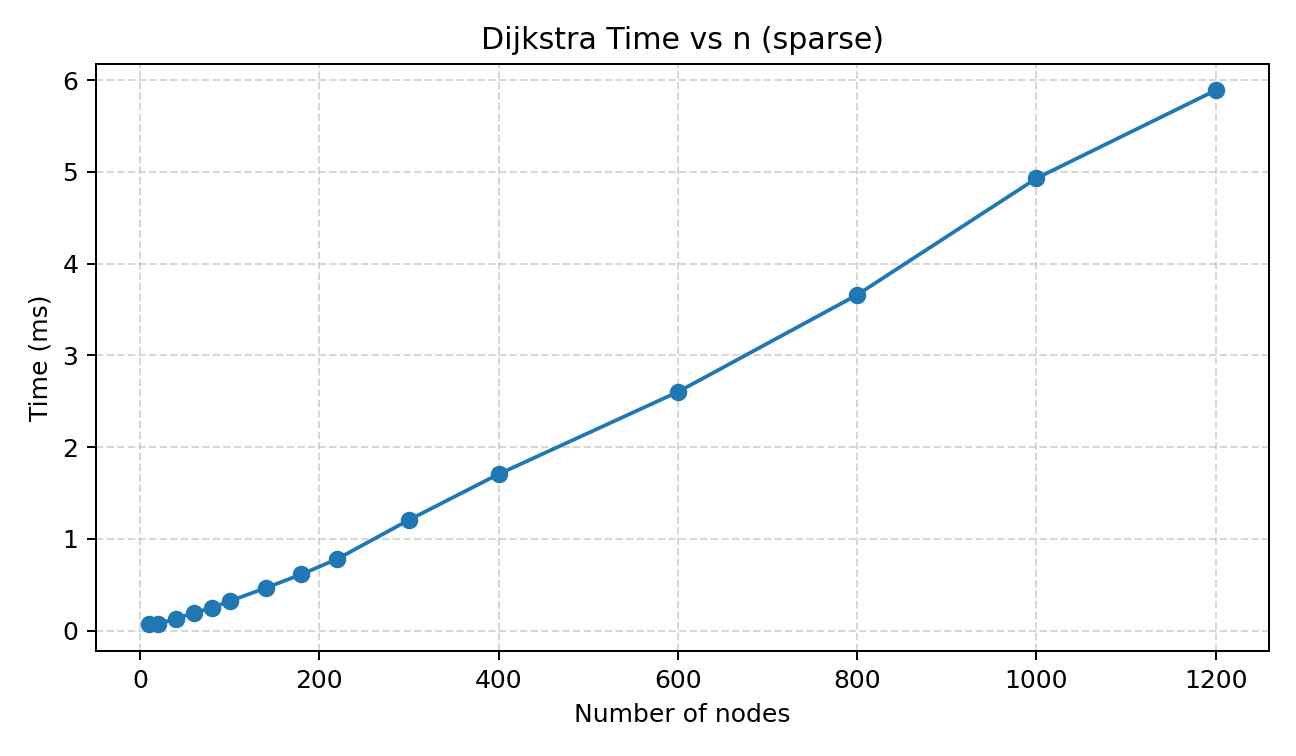
\includegraphics[width=0.48\textwidth]{figures/dijkstra_sparse_time.png}
    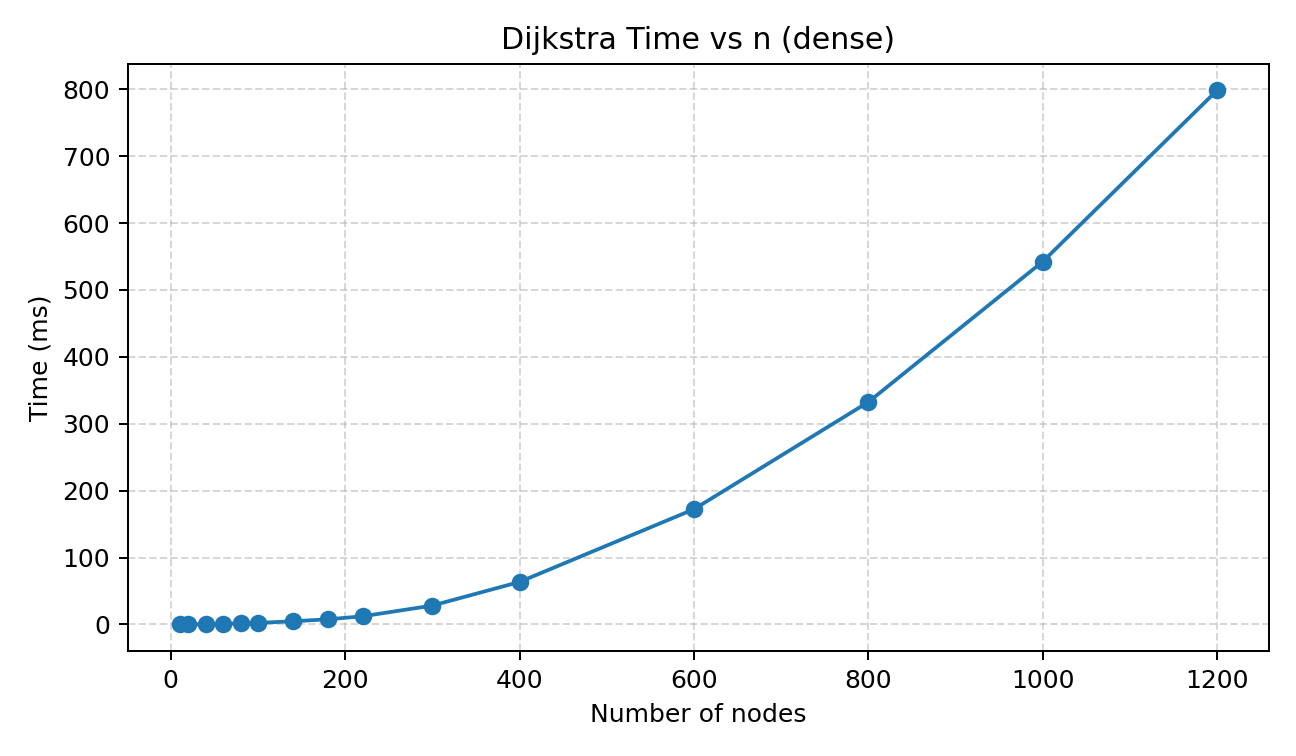
\includegraphics[width=0.48\textwidth]{figures/dijkstra_dense_time.png}
    \caption{Dijkstra: execution time vs number of nodes on sparse and dense graphs}
\end{figure}

\begin{figure}[H]
    \centering
    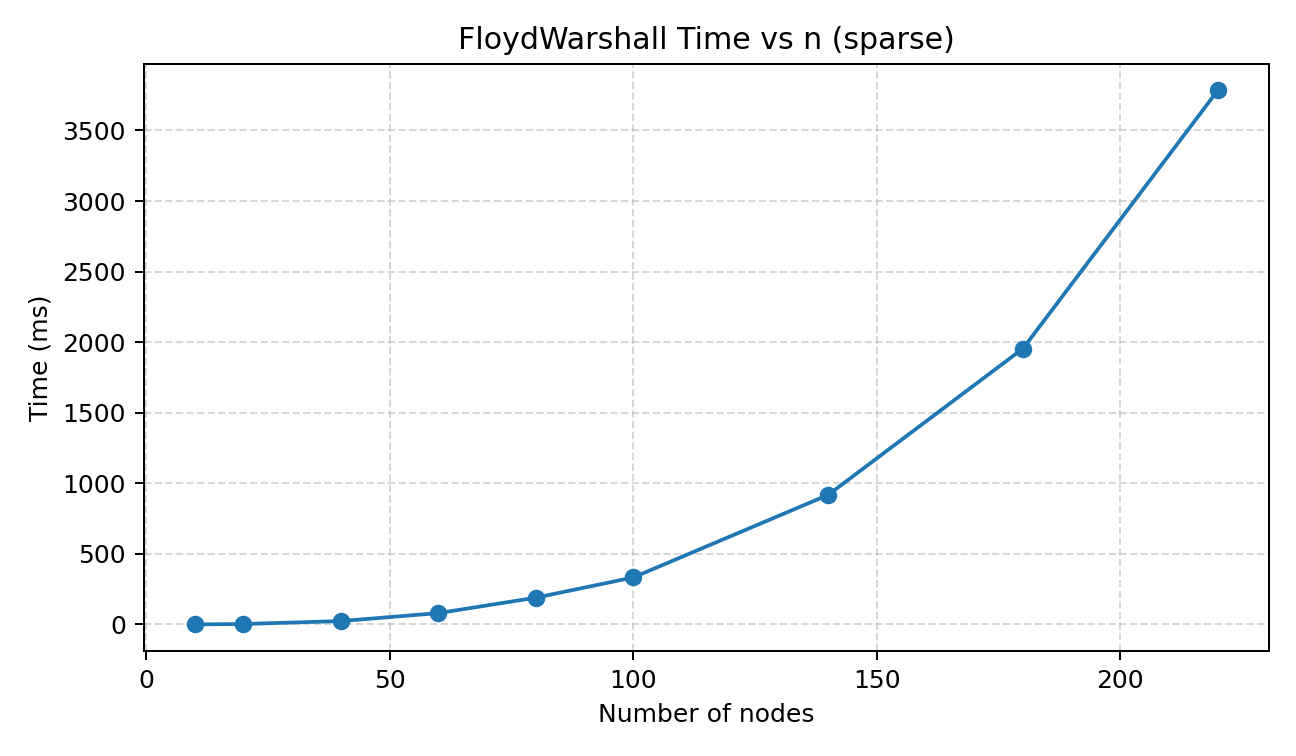
\includegraphics[width=0.48\textwidth]{figures/floydwarshall_sparse_time.png}
    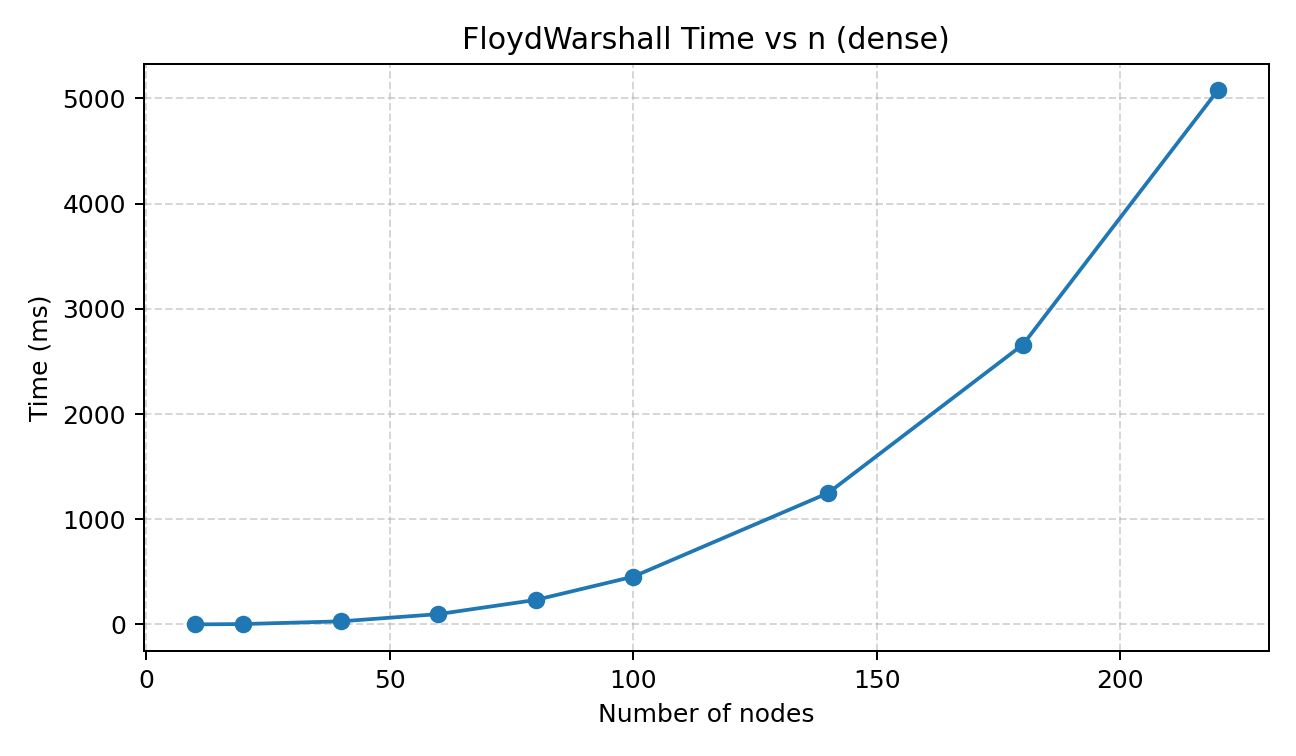
\includegraphics[width=0.48\textwidth]{figures/floydwarshall_dense_time.png}
    \caption{Floyd-Warshall: execution time vs number of nodes on sparse and dense graphs}
\end{figure}

On sparse graphs, Dijkstra clearly dominates. At $n = 100$, Dijkstra is around 0.3 ms while Floyd-Warshall is around 345 ms, a gap above 1000x. Even for very small inputs, Floyd-Warshall is already several times slower. The gap widens as $n$ grows because Dijkstra explores relevant edges, while Floyd-Warshall evaluates all pairs.

The comparison table below gives exact values for selected sizes:

\begin{table}[H]
\centering
\caption{Dijkstra and Floyd-Warshall Comparison (sampled n values)}
\small
\begin{tabular}{llrrrrr}
\toprule
Algorithm & Density & n & m & Time (ms) & Memory (KiB) & Relax attempts\\
\midrule
Dijkstra & dense & 10 & 33 & 0.044 & 0.9 & 33.0\\
Dijkstra & dense & 40 & 523 & 0.376 & 2.1 & 523.0\\
Dijkstra & dense & 100 & 3185 & 2.308 & 4.5 & 3185.0\\
Dijkstra & dense & 220 & 15775 & 12.147 & 9.2 & 15775.0\\
Dijkstra & dense & 600 & 116805 & 172.244 & 24.2 & 116805.0\\
Dijkstra & dense & 1000 & 324918 & 542.354 & 39.9 & 324918.0\\
FloydWarshall & dense & 10 & 33 & 0.401 & 3.2 & 858.0\\
FloydWarshall & dense & 40 & 523 & 29.465 & 46.3 & 62598.0\\
FloydWarshall & dense & 100 & 3185 & 454.166 & 289.4 & 988993.0\\
FloydWarshall & dense & 220 & 15775 & 5077.384 & 1414.4 & 10603772.0\\
Dijkstra & sparse & 10 & 20 & 0.067 & 1.4 & 40.0\\
Dijkstra & sparse & 40 & 80 & 0.130 & 4.0 & 160.0\\
Dijkstra & sparse & 100 & 200 & 0.320 & 9.1 & 400.0\\
Dijkstra & sparse & 220 & 440 & 0.780 & 18.5 & 880.0\\
Dijkstra & sparse & 600 & 1200 & 2.601 & 48.4 & 2400.0\\
Dijkstra & sparse & 1000 & 2000 & 4.930 & 81.2 & 4000.0\\
FloydWarshall & sparse & 10 & 20 & 0.416 & 3.6 & 870.0\\
FloydWarshall & sparse & 40 & 80 & 23.980 & 48.9 & 50354.0\\
FloydWarshall & sparse & 100 & 200 & 332.959 & 308.0 & 722752.0\\
FloydWarshall & sparse & 220 & 440 & 3784.606 & 1501.7 & 7940761.0\\
\bottomrule
\end{tabular}
\end{table}


On dense graphs, Dijkstra still keeps a decisive advantage, although the ratio is smaller. At $n = 100$, Dijkstra is near 2.3 ms versus about 467 ms for Floyd-Warshall. Dense connectivity reduces some wasted work, but all-pairs cubic updates remain much more expensive.

\subsection{Operation Counts and Efficiency}

Execution time can hide implementation details, so operation counts provide a more structural view.

In sparse graphs, Dijkstra performs roughly $O(E)$ relaxations (about $2n$ here), whereas Floyd-Warshall performs $O(V^3)$ pair checks. For $n = 100$, this is about 400 versus 722,000 operations, which explains the large runtime separation.

In dense graphs, Dijkstra's work rises toward $O(V^2)$ as edges increase, while Floyd-Warshall remains cubic, preserving its disadvantage.

\subsection{Memory Footprint}

Memory behavior is also distinct. Dijkstra with adjacency lists uses about $O(V + E)$ memory for graph storage, plus distances and heap. Floyd-Warshall needs $O(V^2)$ space for the distance matrix regardless of sparsity. At $n = 100$, Dijkstra uses about 9 KiB and Floyd-Warshall about 289 KiB. For larger $n$, matrix storage becomes a practical bottleneck.

\begin{figure}[H]
    \centering
    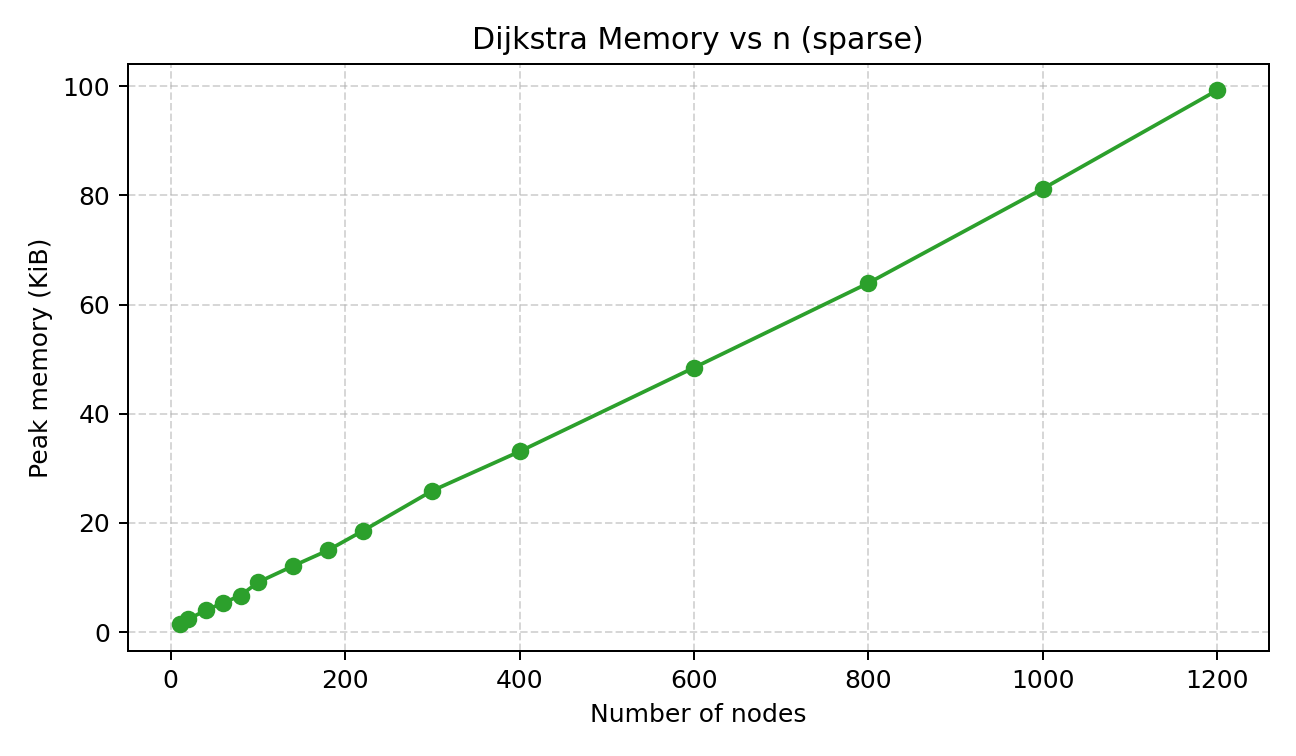
\includegraphics[width=0.48\textwidth]{figures/dijkstra_sparse_memory.png}
    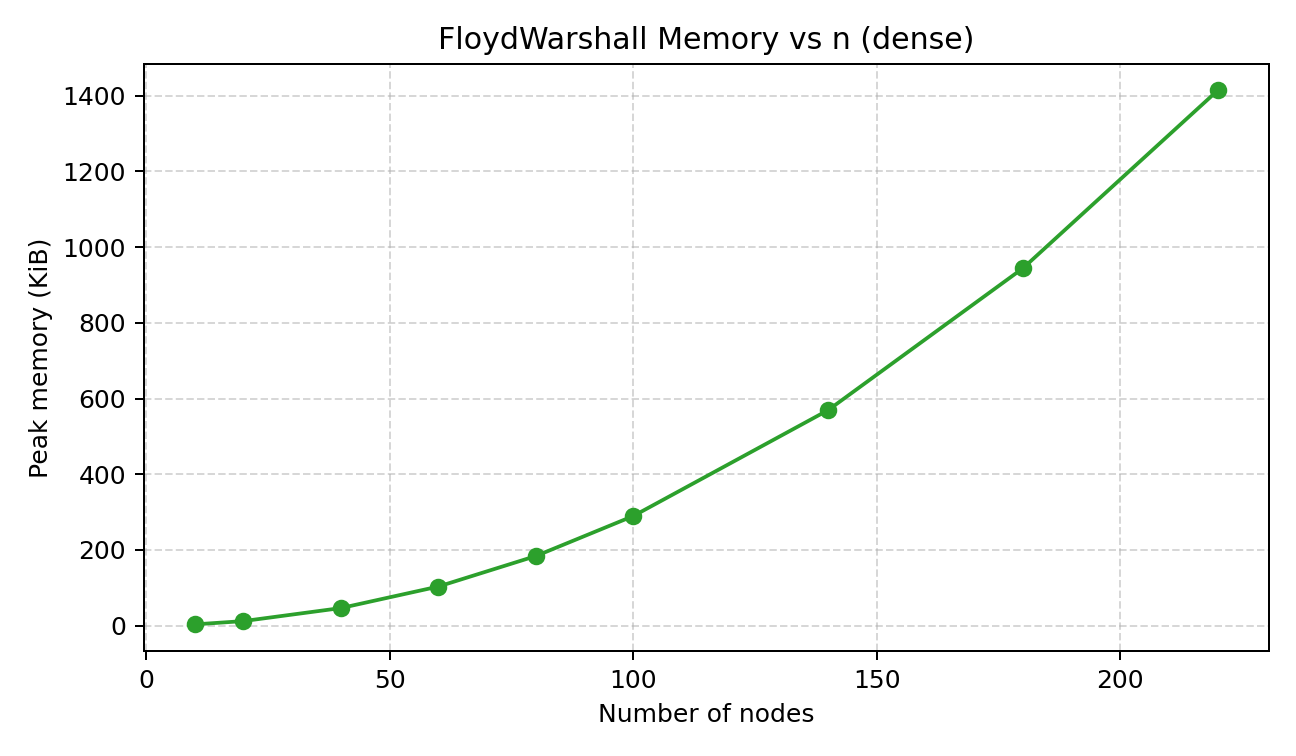
\includegraphics[width=0.48\textwidth]{figures/floydwarshall_dense_memory.png}
    \caption{Memory usage: Dijkstra on sparse graphs and Floyd-Warshall on dense graphs}
\end{figure}

\subsection{Density's Impact}

Graph density changes the two algorithms differently. For Dijkstra, more edges directly increase relaxation work. For Floyd-Warshall, the triple-loop structure dominates regardless of density, so density mainly affects constants.

A practical takeaway is that Dijkstra adapts better across regimes when representation is chosen carefully, while Floyd-Warshall is best reserved for genuine all-pairs workloads.

\section{Conclusion}

The measurements confirm theoretical expectations and add practical guidance. Dijkstra and Floyd-Warshall target different shortest-path settings and should be selected according to query requirements and resource constraints.

For single-source queries, Dijkstra is consistently superior in both sparse and dense tests, often by very large factors. Its cost scales with explored edges, while Floyd-Warshall always pays cubic all-pairs cost.

Floyd-Warshall remains relevant when all-pairs results are required and graph sizes are moderate. In that niche, one full dynamic-programming pass can be justified. However, the $O(V^2)$ memory requirement limits scalability.

Representation choice is also critical. Adjacency lists align with sparse data, while matrix-based operations suit dense processing patterns. The experiment shows that algorithm and data structure decisions are tightly coupled in practice.

A limitation of this work is the use of undirected random-weight graphs and moderate input sizes. Other graph families or directed variants may change constant factors, but the central conclusion remains stable: use Dijkstra for single-source tasks and Floyd-Warshall only when true all-pairs computation is needed on manageable graph sizes.

\newpage

\section{Annex}

GitHub Repository: \url{https://github.com/Lucariowu/aalabs/tree/main/Lab4}

\end{document}
